\section{PathCase KEGG}
\label{sect:pathcase_kegg}

\begin{verse}
    The majority of this section is from ``PathCase: Pathways Database System''
    by ??? \cite{???}.
\end{verse}

\subsection{Overview}
\label{sect:pathcase_overview}

The main goal of PathCase is to provide life scientists with an integrated
environment to study pathways, regardless of the source producing the
corresponding data. More specifically, rather than becoming an ultimate and
authoritative data source for pathways, PathCase’s vision is to become a
powerful, data source-independent, one-stop computational environment
encapsulating an extensive set of tools for systems-level research on cellular
actions. To this end, PathCase emphasizes six distinct dimensions as the focus
of the overall system: (1) storing, (2) analyzing, (3) visualizing, (4)
querying, (5) modeling, and (6) sharing pathways data.

\begin{enumerate}

    \item \textbf{Storage}: PathCase runs on a relational database, and the web
    content is dynamically created using the compiled data from the database.
    The main data objects are pathways, processes, and molecular entities. To
    increase the efficiency of queries and web page content retrieval, the
    database employs a large number of indices defined on groups of database
    attributes.  Some fields (e.g., links between pathways) are pre-computed to
    improve the response time.

    \item \textbf{Analysis}: PathCase provides tools for the analysis of
    pathways at various levels of granularity in different dimensions. PW-ANN is
    one such tool. Another tool takes any user-provided set of genes, and
    retrieves a set of pathways that are tightly associated with the input
    genes. A third tool allows pathway analysis in terms of the locations of
    genes encoding the enzymes of its processes to see how closely they are
    located on a given genome. 

    \item \textbf{Visualization}: PathCase has a powerful visualization tool
    with advanced, flexible, automated layout generation engine. Pathways can be
    visualized at different detail levels, such as the expanded-form, which
    displays all the components of a pathway (from reactions to activators) and
    the collapsed form, which is used to visualize the connections between
    pathways in a compact way. In addition, PathCase also visualizes a large
    number of query results. All the visualizations are created dynamically (at
    the client side), and can be edited by users.  

    \item \textbf{Querying and Browsing}: PathCase puts an extensive emphasis on
    querying and browsing the underlying pathways data in an effective way.
    Users can either use powerful built-in queries to pose various queries from
    path-finding between two molecules to locating neighbors of a pathway in a
    metabolic network. When pre-defined built-in queries are not sufficient to
    perform to the user’s task at hand, the Advanced Query Interface (AQI)
    allows users to build their own queries in a flexible and user-friendly way.
    Alternatively, for users who are browsing and do not yet know what they are
    looking for, PathCase provides an elegant browser for each biological entity
    type, e.g., organisms, proteins, reactions.

    \item \textbf{Modeling}: In PathCase, pathways are represented as
    hypergraphs \cite{Berge-1973} where nodes are molecular entities
    participating in a reaction as substrates or products, and edges are enzymes
    which catalyze reactions. Moreover, PathCase also models pathways as a graph
    of Gene Ontology (GO) functional annotations, called \emph{pathway
    functionality templates}, where each node corresponds to a GO annotation of
    an enzyme catalyzing a process. For a given pathway, different functionality
    templates can be created by using the generalization/specialization
    hierarchy of the GO.

    \item \textbf{Sharing}: PathCase provides three distinct mechanisms to share
    its data and visualizations with the scientific community: (i) all pathways
    can be exported to BioPAX formatted documents \cite{BioPAX}, (ii)
    visualizations can be saved in an image format (JPEG), and (iii) PathCase
    web service methods can be directly accessed in order to query the PathCase
    database and obtain the results in XML format. PathCase can also import
    BioPAX-formatted pathway documents, and visualize them.

\end{enumerate}

\textbf{PathCase KEGG} is the version of PathCase that is modeled on pathways
from KEGG.

\subsection{System Architecture}
\label{sect:pathcase_architecture}

The PathCase system architecture, shown in figure
\ref{fig:pathcase_architecture}, has four distinct layers. Starting with the
server side, the first layer consists of the databases, which contain the actual
pathways information and allow for efficient querying.

\begin{figure}[hbt]
    \center{
        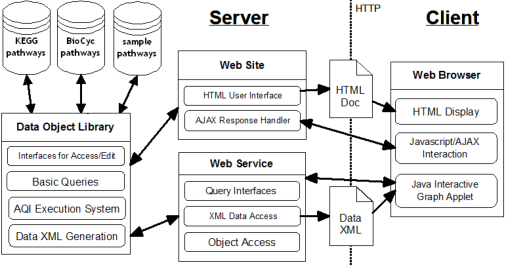
\includegraphics[width=4in]{background/figures/architecture.pdf}}
    \caption{\label{fig:pathcase_architecture} PathCase system architecture}
\end{figure}

The next layer is the data object library, which provides a programmer-friendly
interface to the system content stored in the databases that allows for data to
be accessed, created, and updated.

The next layer, the web server, includes the PathCase web site and the web
service, which generates HTML pages and XML data.

The final layer, on the client side, includes the components of PathCase that
run on the user’s web browser. This includes the HTML, CSS and Javascript, as
well as the graph viewer java applet used for interactive pathway graph
visualization.

The graph viewer applet makes use of the web service component in order to
request additional data as needed, and enhance the graph visualization without
requiring the user to reload the web page. All graph manipulations such as
zooming in and out, panning, and application of different layouts are carried
out on the client side with no server side requests.

\subsection{Data Model}
\label{sect:pathcase_data_model}

In the PathCase data model, we represent a metabolic pathway \cite{Michal-1999} in
the form of a graph where nodes represent molecules, and edges represent
reactions (or processes) connecting the molecules that take part in the
reaction. As reactions may involve more than one substrate and more than one
product, the reaction is actually a hyper-edge, and a pathway is a hyper-graph
\cite{Berge-1973}. We use the term process to denote reactions, which can include a
catalyzing protein (which also identifies the reaction and may have an enzyme
classification number), co-factors, inhibitors and activators. Reactions may be
one-way or reversible. We refer to molecular objects as molecular entities which
include basic molecules, proteins, enzymes, genes, and amino acids. A pathway
can be viewed as a set of interconnected processes, while a process can be
viewed as being made up of molecular entities. More generally, an entire
pathways database can be viewed as a single large graph of interconnected
reactions, in which certain sub-graphs are identified as specific pathways. This
way, the system can dynamically visualize, query, and analyze any subsection of
the larger pathways network, or even show how pathways themselves are
interconnected at a higher level. Connected pathways are pre-calculated for
efficient querying and visualization. Pathways are also organized into pathway
groups, representing a set of pathways with related functionality. 

The PathCase model also maintains the organism in which a process occurs.  This
allows the user to switch from viewing a general pathway graph to viewing its
organism-specific version, in which the components that do not apply are
dynamically grayed out.  Organisms can be organized into a hierarchy of organism
groups, allowing for easy visualization of the pathway for an entire kingdom,
phylum, etc.  Organisms can also be associated with chromosomes, and store the
location of genes that encode proteins. This enables the user to quickly find
gene and chromosome location for a process’ catalyzing protein and vice versa.
